\chapter{The CMS experiment at the LHC}
\label{sec:cms}

\section{The Large Hadron Collider}

The Large Hadron Collider (LHC)~\cite{lhcjinst}\footnote{Unless otherwise specified, all technical specifications of the LHC are derived from Reference~\cite{lhcjinst}} is a circular particle accelerator, 27 km in circumference and between 40 and 175 m below the surface of the French-Swiss border. 
Designed to collide protons at a maximum center-of-mass energy $\sqrt{s} = 14$ TeV, the LHC has delivered collisions at $\sqrt{s}=7,8$ TeV (Run 1) and $\sqrt{s} = 13$ TeV (Run 2); the target energy $\sqrt{s} = 14$ TeV will be reached in Run 3. 
In addition to protons, the LHC accelerates and collides heavy nuclei (Pb and Xe) at lower values of $\sqrt{s}$. 
In this thesis, we focus exclusively on data recorded from proton collisions during Run 2. 

\begin{figure}[]
    \begin{center}
        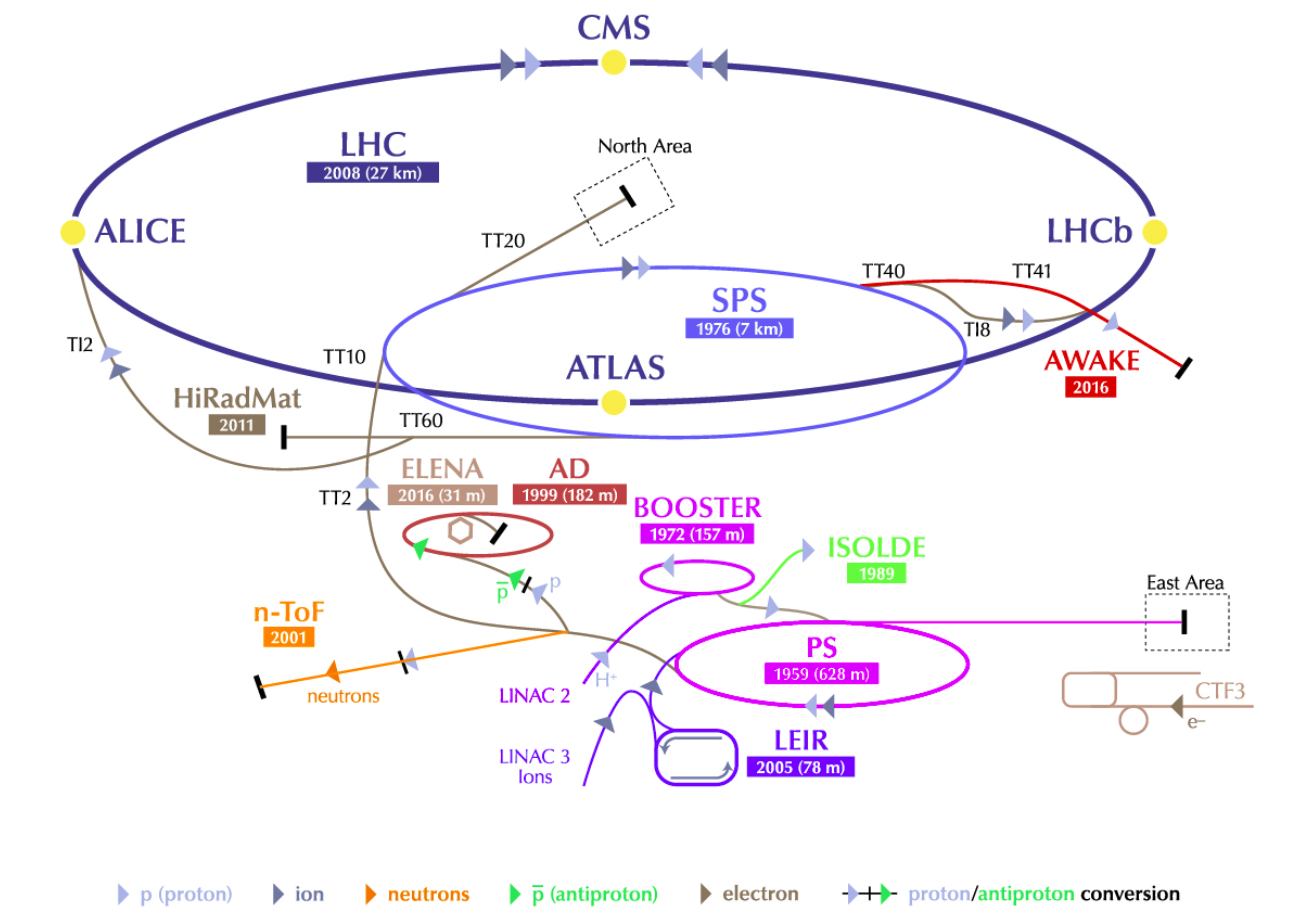
\includegraphics[width=0.8\textwidth]{figures/cms/lhc.png}
        \caption{Diagram of the CERN accelerator complex.
                 The LHC (dark blue) is fed protons (and heavy ions) by a chain of intermediate accelerators, beginning with LINAC2 (dark pink).i
                 Reprinted from Reference~\cite{lhcpic}. 
                    }
        \label{fig:cms:lhc}
    \end{center}
\end{figure}

Protons are brought to the LHC by the multi-stage process~\cite{lhctdr3} depicted in Figure~\ref{fig:cms:lhc}.
Hydrogen atoms are stripped of electrons and accelerated by LINAC2 (a linear accelerator) to a kinetic energy of $50$ MeV.
LINAC2 then feeds the protons into the Booster ring (final energy of $1.4$ GeV), followed by the Proton Synchrotron ($26$ GeV).
From the PS, the protons are injected into the Super Proton Synchrotron ($450$ GeV).
Protons exit the SPS and enter the LHC at one of two places, corresponding to two different beams traveling in opposite directions.
The two beams intersect in eight places along the LHC, four of which are instrumented by a detector experiment: CMS, ATLAS, LHCb, and ALICE. 

Each proton beam in the LHC is accelerated by eight superconducting cavities exerting radio frequency longitudinal (i.e. parallel to beam direction) electric fields with a frequency of $400$ MHz,
The maximum RF voltage seen by each beam is 16 MV per revolution.
The physical and temporal design of the RF system creates bunches of protons (corresponding to nodes of the oscillating field) approximately 7.5 cm in length and separated by 25 ns. 
Superconducting NbTi dipole magnets bend the two proton beams in opposite directions as they travel around the ring. 
Each of the 1232 dipoles is 14 m long and exerts a transverse $B$ field between $0.54$ and $8.33$ T.
To achieve such high $B$ fields, the magnets are cooled to 2 K by superfluid helium.
In addition, a number of quadrupole magnets are used to focus and match the beams between the dipoles\footnote{Full details on the various quadrupoles can be found in Table 3.7 of Reference~\cite{lhcjinst}.}.

In addition to the center-of-mass energy $\sqrt{s}$, the other figure of merit is the number of events producing interesting physics processes, which is defined as:
\begin{equation} 
    N(pp\rightarrow X) = \int dt L \sigma(pp\rightarrow X)
\end{equation}
where $\sigma$ is the cross section of the relevant process and $L$ is the instantaneous luminosity of the LHC. 
The cross section is fixed by nature, and so increasing the luminosity is the only handle to increase $N$. 
The instantaneous luminosity of two Gaussian beams is given by~\cite{lhcjinst}:
\begin{equation}
    L = \frac{N_b^2 n_b f_\mathrm{rev} \gamma F}{4\pi\epsilon \beta^*}
\end{equation}
where:
\begin{itemize}
    \item[$N_b$ $=$] particles per bunch
    \item[$n_b$ $=$] bunches per beam 
    \item[$f_\mathrm{rev}$ $=$] frequency of revolution 
    \item[$\gamma$ $=$] $E/m$ of beam 
    \item[$\epsilon$ $=$] emittance of beam 
    \item[$\beta^*$ $=$] beta function at collision point 
    \item[$F$ $=$] factor accounting for beam intersection geometry
\end{itemize}
The instantaneous luminosity evolves as a function of time, primarily due to $n_b$ and $N_b$ being modified by collisions.
The total integrated luminosity after time $T$ is:
\begin{equation}
    L_\mathrm{int} = \int_0^T dt L(t) = L(0) \tau_L \left(1 - e^{-T/\tau_L}\right)
\end{equation}
where $\tau_L \approx 15$ h is the characteristic beam loss timescale and $L(0)$ is the instantaneous luminosity at $T=0$.
The LHC is designed to deliver $L(0) \sim \mathcal{O}(10^{34})$ cm$^{-2}$s$^{-1}$. 
Figure~\ref{fig:cms:lumi} shows the total luminosity delivered by the LHC and recorded by CMS during the 2016 portion of Run 2. 

\begin{figure}[]
    \begin{center}
        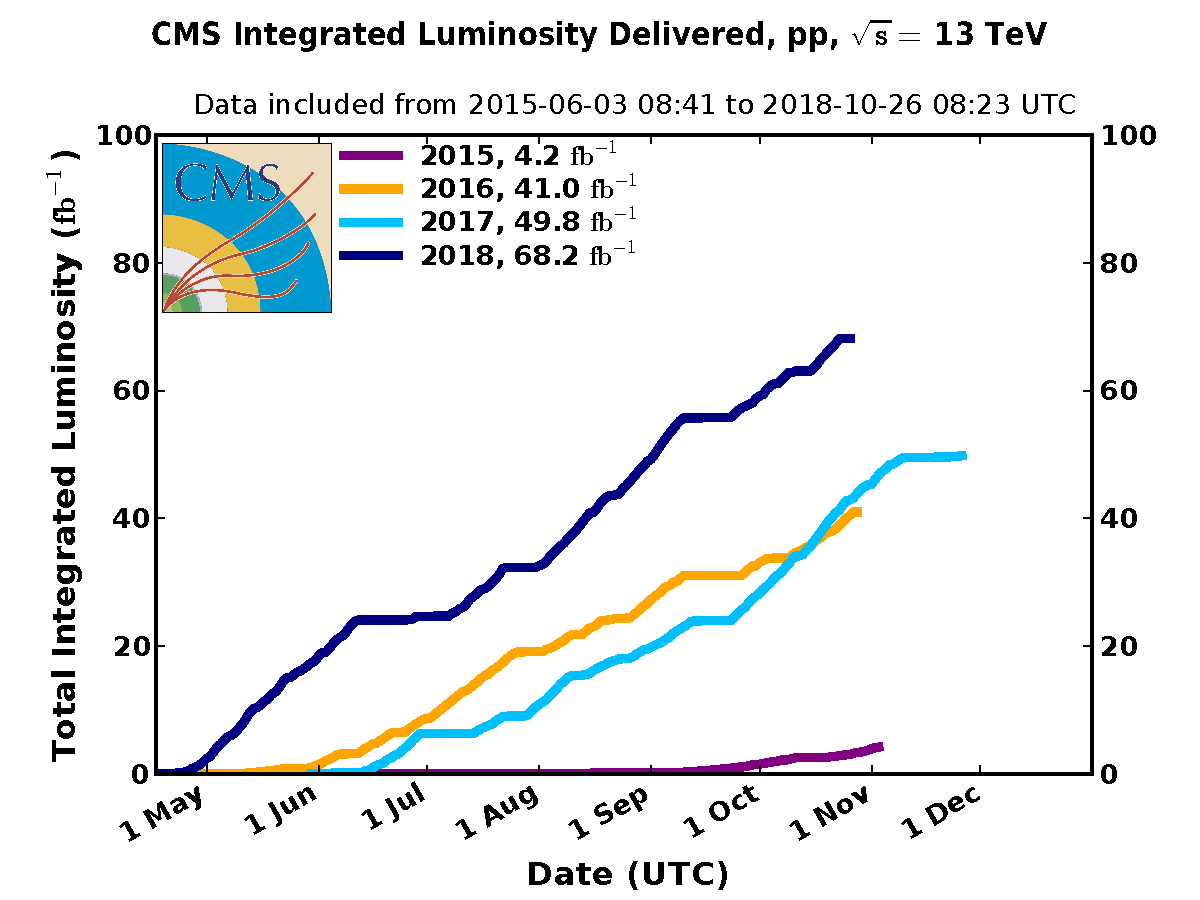
\includegraphics[width=0.5\textwidth]{figures/cms/lumi.pdf}
        \caption{Integrated luminosity of the LHC during proton collisions during the 2016 data-taking period~\cite{lumitwiki}.}
        \label{fig:cms:lumi}
    \end{center}
\end{figure}

\section{The Compact Muon Solenoid}

The Compact Muon Solenoid (CMS)~\cite{cmsjinst} is one of two general purpose LHC detectors (the other being ATLAS).
It is designed to detect and measure stable hadrons, photons, electrons, and muons produced in proton and ion collisions at LHC interaction point 5. 
From these event descriptions, a number of physics processes can be probed, including SM measurements~\needcite, BSM searches~\needcite, and the discovery of the Higgs boson~\needcite. 
In what follows, we will use the $(r,\phi,\eta)$ coordinate system with respect to the $z$ axis:
\begin{itemize}
    \item[$z = $] distance along beam axis, with $z=0$ defined to be at the center of the detector
    \item[$r = $] distance from the $z$ axis
    \item[$\phi = $] azimuthal angle in the plane orthogonal to the $z$ axis
    \item[$\eta = $] pseudorapidity $(-\log\nicefrac{\theta}{2}$), with respect to the polar angle $\theta$ 
\end{itemize}
In this coordinate system, we define $x$ and $y$ to lie in the plane perpendicular to $z$, with $x$ pointing from the center of the detector to the center of the LHC.
As with the pseudorapidity, it is convenient to use quantities invariant under $z$-boosts, and so we define the transverse momentum:
\begin{equation}
    \vec{p}_\mathrm{T} = \left(\begin{matrix} p_x \\ p_y \end{matrix}\right)
\end{equation}
We will frequently make use of the magnitude of this vector, $\pt$. 
CMS can detect collision products that are within the fiducial volume of $0 \leq \phi < 2\pi$ and $-5 \leq \eta\leq 5$. 
Several detector subsystems (Figure~\ref{fig:cms:cms}) are used to identify and reconstruct muons, electrons, photons, and charged and neutral hadrons. 

\begin{figure}[]
    \begin{center}
        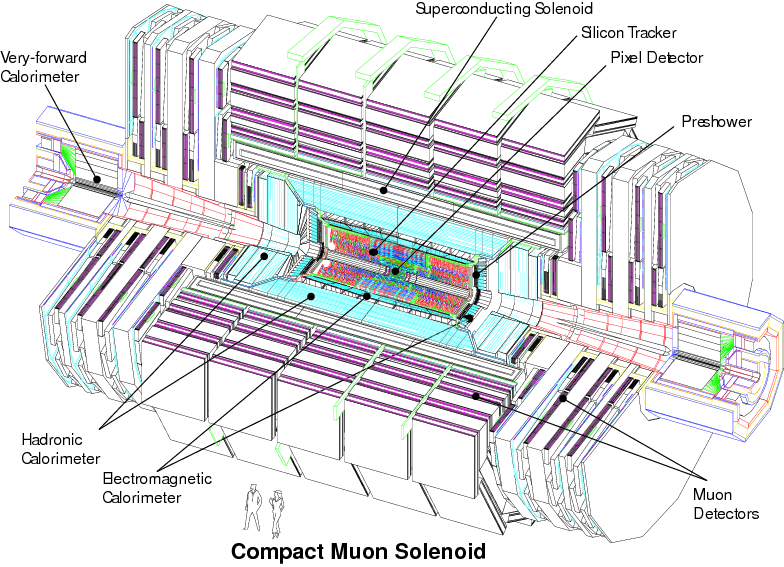
\includegraphics[width=0.65\textwidth]{figures/cms/cms.png}
        \caption{Cut-away view of the CMS detector and its subsystems.
                 Reprinted from Reference~\cite{cmsjinst}.}
        \label{fig:cms:cms}
    \end{center}
\end{figure}

\subsubsection{Silicon tracker}

Starting from the beam pipe, the first of these subsystems is the silicon tracker~\cite{cmstracker}, used to identify charged particles and measure their momenta. 
The tracker consists of silicon detector geometries: pixels (providing 3D position measurement) and strips (2D). 
The arrangement of the pixel and strip layers are shown in Figure~\ref{fig:cms:si}.
A near-uniform 3.8 T magnetic field, produced by a superconducting NbTi solenoid, envelopes the tracker. 
The field lines in the tracker volume are approximately parallel to the beam direction. 

A single silicon pixel has dimensions $285\times100\times150$ $(\mu\mathrm{m})^3$ (in $r\times r\phi\times z$), leading to a position resolution of $\sim10\times30$ $(\mu\mathrm{m})^2$ (in $r\phi\times z$). 
The 66 million pixels are arranged into 7 layers: 3 cylindrical ``barrels'' (at $r=4.4,~7.3,~10.2$ cm) and $2\times2$ ``endcap'' annulli (at $z=\pm34.5,~\pm46.5$ cm). 
Outside the pixel layers are the strip layers, consisting of 9.3 million silicon strips arranged into barrels and endcaps.
The resolution in $r\phi$ varies between $10$ and $50$ $\mu$m, depending on the location and pitch of the given strip.
Certain strip layers contain two layers of strips, rotated through a ``stereo'' angle (100 mrad) with respect to each other.
By matching adjacent hits, the stereo measurement can add a third dimension ($z$ for barrel, $r$ for endcap) to the strip's 2D measurement, with resolution $100$-$500$ $\mu$m.
There are a total of 10 barrel layers ($0.2 < r < 1$ m) and 24 endcap layers ($0.6 < |z| < 2.8$ m). 

\begin{figure}
    \begin{center} 
        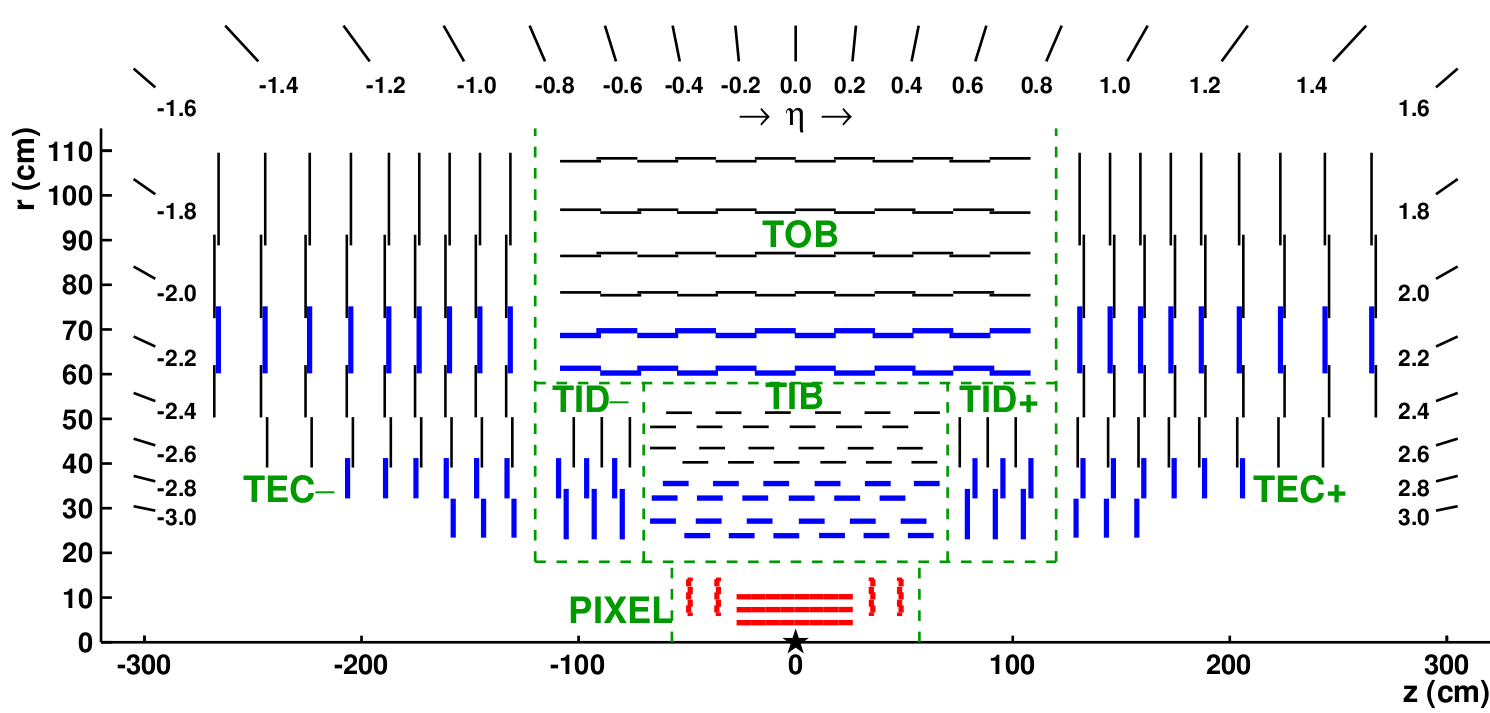
\includegraphics[width=0.7\textwidth]{figures/cms/tracker.png}
        \caption{Diagram of a slice of the CMS tracking system.
                 The pixel layers are shown in bold red lines.
                 Single-strip (double-strip) layers are indicated by thin black (bold blue) lines.
                 The double-strip modules each consist of two back-to-back strips, rotated with respect to each other, that can provide 3D localization of the hits.
                 Reprinted from Reference~\cite{cmstracker}.}
        \label{fig:cms:si}
    \end{center}
\end{figure}

Pixels with a signal greater than a tuneable readout threshold (typically around $3000 Q_e$) are read out.
These pixels are then aggregated with adjacent signals to form pixel clusters, which are further subjected to readout thresholds ($\sim 4000 Q_e$).
The exact position of the particle in this layer (known as a ``hit'') is inferred by fitting the charge distribution of the pixels in this cluster to pre-determined templates.
A similar method is employed to determine the strip hit positions, with some modifications to account for Lorentz drift of the charges in the silicon detector due to the $B$-field. 
The efficiency of reconstructing hits varies with the detector type, location, and particle momentum, but is generally greater than $99\%$ ($99.5\%$ if defective modules are not considered). 

Tracks are found using an iterative ``inside-out'' process, where each iteration has five steps:
\begin{enumerate}
    \item Define seeds using pixel hits, double-strip hits (i.e. hits with 3D information), and an estimate of the beam spot (collision point). At least 3 hits are needed for the seed.
    \item Use a Kalman filter~\needcite to evolve track seeds through the rest of the tracker and find hits, accounting for the $B$-field and energy loss.
    \item Estimate trajectory parameters after finding all hits.
    \item Decide whether to keep found tracks based on quality requirements (e.g. number of missing hits, track $\chi^2$)
    \item Remove hits associated with tracks from hit collection and repeat.
\end{enumerate}
The trajectory parameters referred to in step 3 are the 5 parameters of a helix: $\rho$ (curvature), $\phi_0$ (azimuthal angle), $\lambda$ ($\cot\theta$), $d_0$ (``impact parameter'', minimum $r$ of track), $z_0$ (minimum $|z|$ of track).
The CMS track fit typically has 5-7 iterations, with each successive iteration loosening the seed and track fit requirements to look for more difficult tracks (e.g. missing hits, large $d_0$).
The efficiency and fake rate of this reconstruction, as a function of track \pt, are shown in Figure~\ref{fig:cms:trackeff}.
For muons with $|\eta|<1.5$ and $\pt>1$ GeV, the tracking efficiency is over 98\%, with a combinatorial fake rate of 2-6\%. 

\begin{figure}
    \begin{center} 
        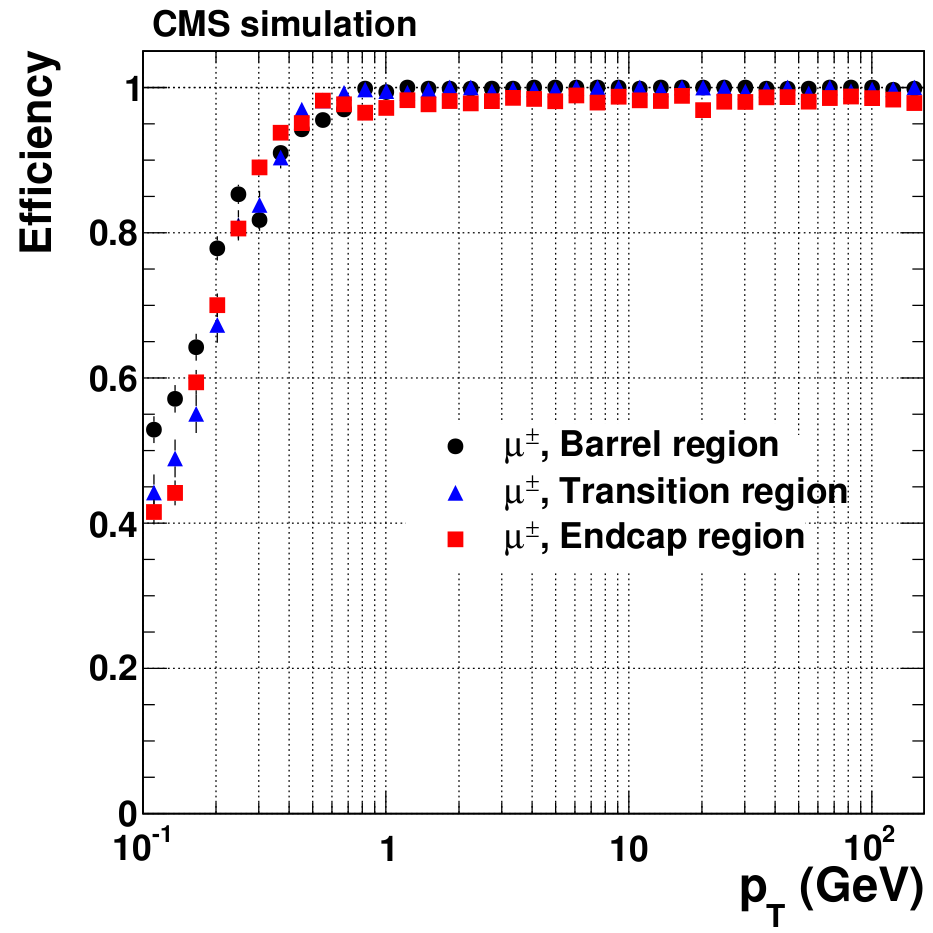
\includegraphics[width=0.35\textwidth]{figures/cms/track_eff.png}
        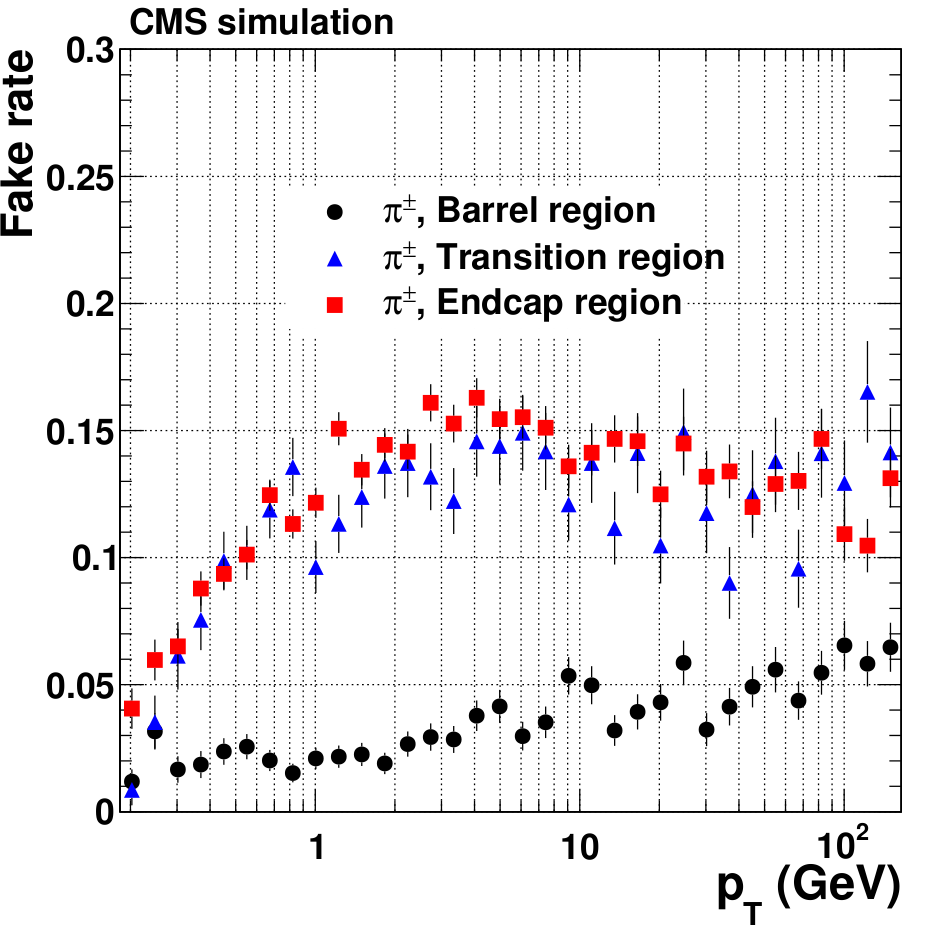
\includegraphics[width=0.35\textwidth]{figures/cms/track_fake.png}
        \caption{Efficiency (fake rate) of the CMS track fit algorithm, evaluated using simulation of muons (charged pions).
                 Reprinted from Reference~\cite{cmstracker}.}
        \label{fig:cms:trackeff}
    \end{center}
\end{figure}

The excellent position resolution of the pixel detector is used to accurately measure the position of primary vertices, as well as any secondary vertices from the decays of long-lived particles.
In the former case, tracks are first clustered together on the basis of the likelihood that the tracks in a cluster arise from a single primary vertex.
This is done using a deterministic annealing algorithm~\cite{da}, which has as free parameters the number of clusters and the probability of each track belonging to each cluster.
Having determined the clusters, an adaptive fit algorithm~\cite{adaptivefit} is used to determine the vertex for each cluster.
The free parameters of this fit are the three spatial coordinates of the vertex.
As the LHC collides bunches of $\mathcal{O}(10^{11})$ protons, we expect multiple primary vertices in a single collision, and this is reflected in Figure~\ref{fig:cms:npv}.
The vertex defined to be the hard scattering interaction (known as \emph{the} primary vertex\footnote{This nomenclature is indeed confusing, defining the singular primary vertex to be one of many primary vertices. However, it is standard terminology in CMS publications, so we will continue to use it. In what follows, the distinction will be clear}) is the vertex which maximizes:
\begin{equation}
	\sum_{j\in\mathrm{track jets}} (\pt^j)^2 + (\ptmiss)^2
\end{equation}
where ``track jets`` refer to jets (Section~\ref{sec:cms:jets}) clustered from the vertex's tracks, and \ptmiss~is defined in Section~\ref{sec:cms:met}.

\begin{figure}
    \begin{center} 
        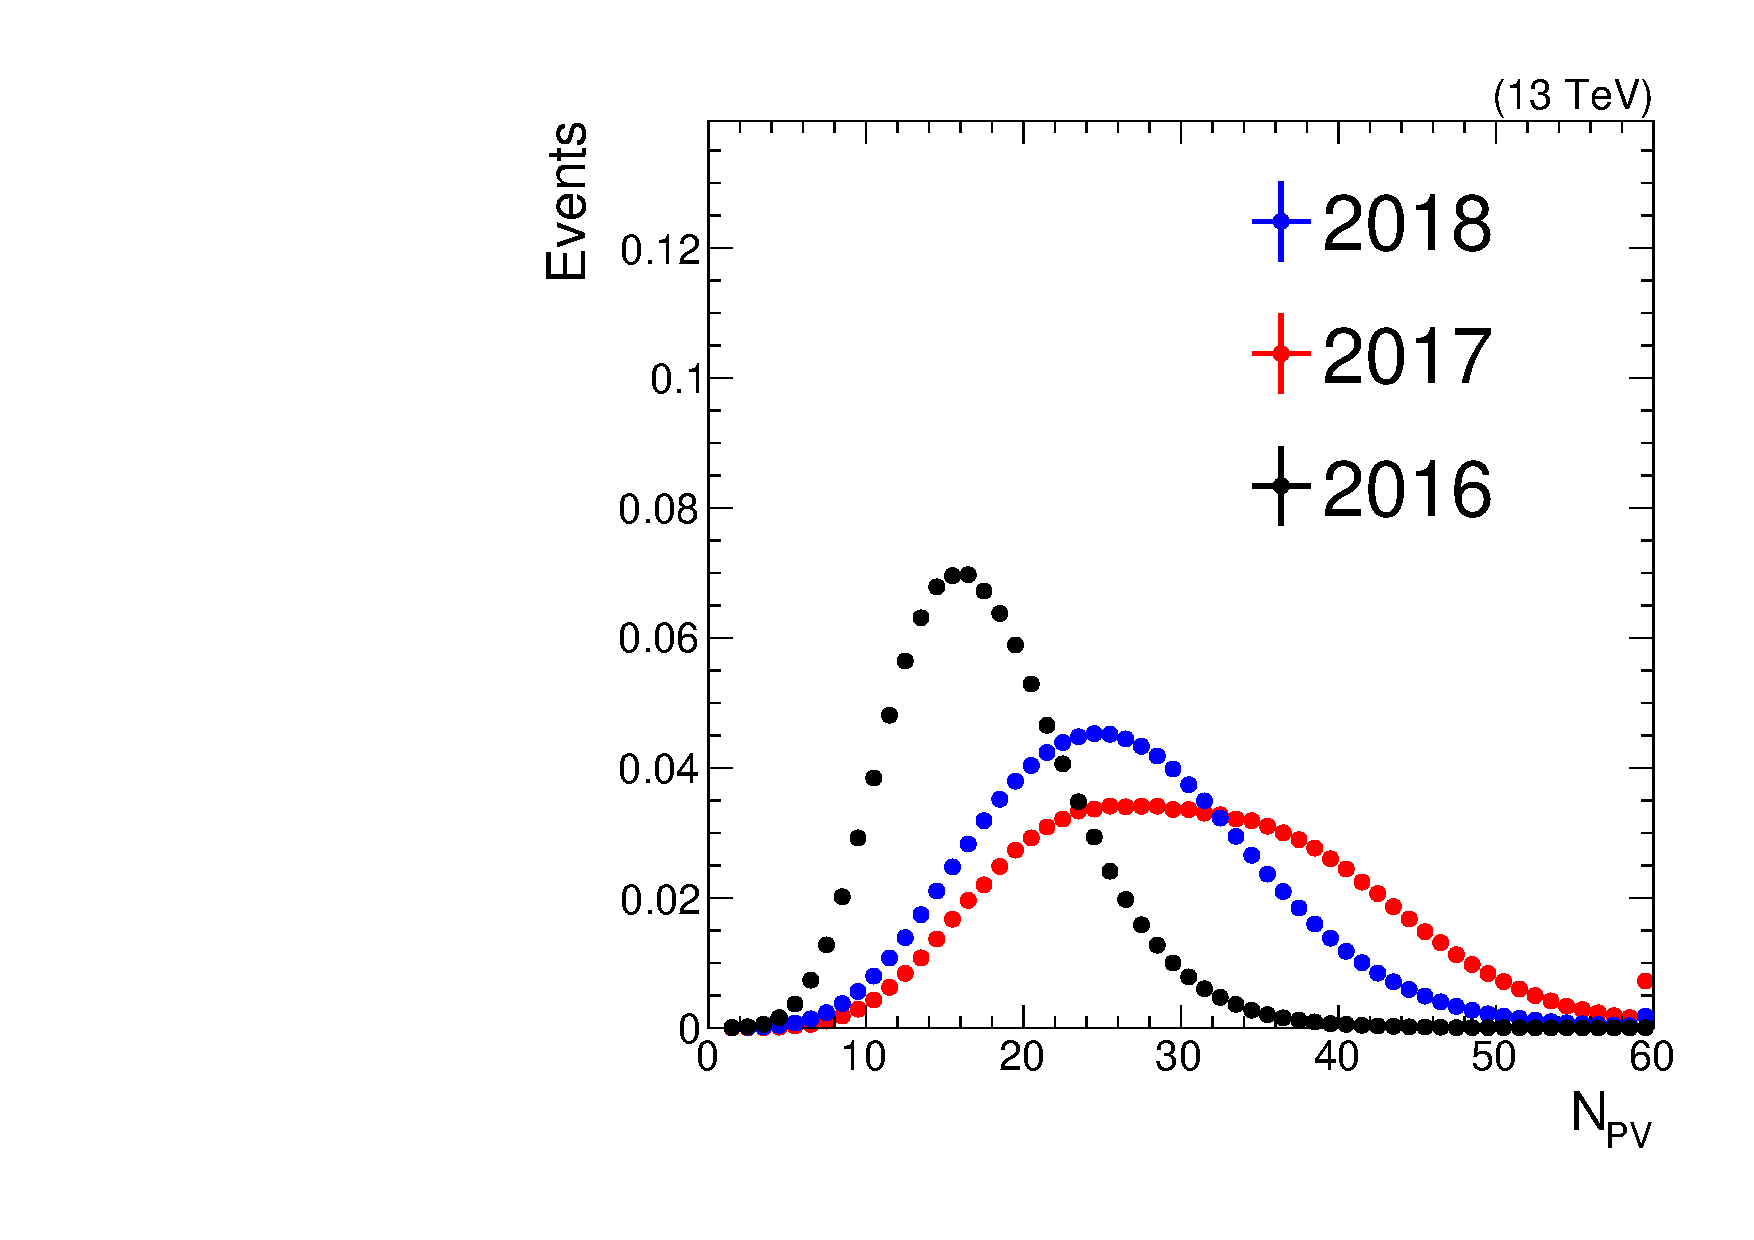
\includegraphics[width=0.7\textwidth]{figures/cms/comparison_npv.pdf}
        \caption{The distribution of the number of reconstructed primary vertices in data recorded by CMS during Run 2 of the LHC.
				 While the results in this thesis only concern 2016 data, we show the evolution of $N_\mathrm{PV}$ as a function of time, as this correlates directly with increased instantaneous luminosity.}
        \label{fig:cms:npv}
    \end{center}
\end{figure}

The last reconstruction algorithm concerning the tracker alone is the identification of secondary vertices, which arise from the decay of long-lived particles (e.g. $B$ mesons).
The inclusive vertex fitter (IVF)~\cite{csvv2} reconstructs such secondary vertices by the following steps:
\begin{enumerate}
	\item Select a track as a seed if it satisfies $\sqrt{d_0^2 + d_z^2} > 50~\mu\mathrm{m}$ and $d_0 > 1.2 \delta d_0$.
	\item Choose nearby tracks based on their closest distance to and opening angle with the seed track.
	\item Fit the tracks to a displaced vertex using the adaptive fitter~\cite{adaptivefit}.
	\item Decide which tracks belong to the candidate secondary vertex and which belong to the primary vertex.
	\item Re-fit the secondary vertex position only using the former set of tracks from the previous step.
\end{enumerate}
It is important not only to properly determine the location of the secondary vertex, but also to properly assign tracks.
Observables that are a function of the \emph{tracks} (e.g. vertex mass) will be critical for $b$ jet tagging.

\subsubsection{Electromagnetic calorimeter}

The CMS electromagnetic calorimeter~\cite{cmsecaljinst} (ECAL) is a homogenous detector with good energy and angular resolution, composed of 76,000 \pbwo~crystals. 
The crystals are arranged in two sections: a cylindrical barrel (EB) covering $|\eta|<1.44$ and two endcap annuli (EE) extending to $|\eta|<3$.
This provides slightly more coverage than the tracking volume.
Each crystal in the EB (EE) has dimensions $2.2\times2.2\times23$ ($2.68\times2.68\times22$) $(\mathrm{cm}^3)$, with the long dimension pointing towards the beam.
This can be compared to a Moli\'ere radius $r_M=2.19$ cm and a radiation length of $X_0=0.89$ cm. 
A cross-sectional area comparable to $r_M\times r_M$ facilitates the differentiation of different electromagnetic (EM) showers arising from electrons and photons.
The depth of the crystal (in units of $X_0$) drives the excellent energy resolution, which is determined using a electron beam:
\begin{equation}
    \frac{\sigma_E}{E} = \frac{2.8\%}{\sqrt{E/\mathrm{GeV}}} \oplus \frac{12\%}{E/\mathrm{GeV}} \oplus 0.3\%
\end{equation}
Scintillation photons from the \pbwo~crystals are collected by avalanche photodiodes (APDs) in the EB and vacuum phototriodes (VPTs) in the EE, which provide amplification factors of 50 and 10, respectively. 

At high momenta, the two photons from a $\pi^0$ decay may merge into a single ECAL crystal. 
This primarily occurs at high $|\eta|$ due to the $z$-boost of the intitial state.
To differentiate one- and two-photon deposits, a ``preshower'' detector sits in front of the EE ($1.6 < |\eta|<2.5$).
The preshower detector consists of a lead absorber and silicon strips.
A photon (or photon pair) initiates a shower in the lead.
The shower can be resolved in the silicon strips, which have resolution $\mathcal{O}(1\mathrm{-}10)$ mm.

The physical placement of all three ECAL components is shown in Figure~\ref{fig:cms:ecal}.

\begin{figure}
    \begin{center} 
        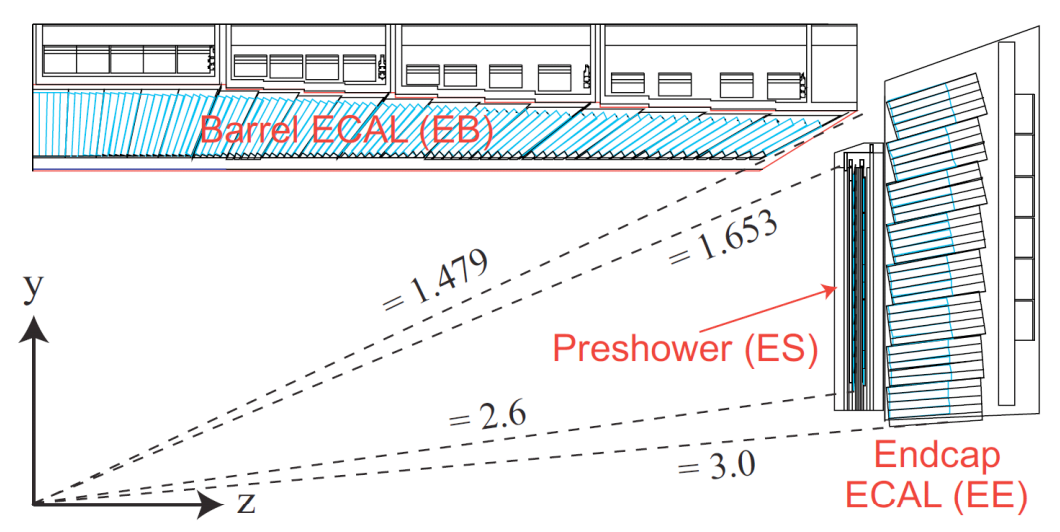
\includegraphics[width=0.7\textwidth]{figures/cms/ecal.png}
        \caption{One quadrant of the CMS ECAL (symmetric with rotation around $z$ and reflection across $z=0$).
                 The dashed lines indicate values of $\eta$.
                 Reprinted from Reference~\cite{cmsecaljinst}.}
        \label{fig:cms:ecal}
    \end{center}
\end{figure}

Due to the bending of a charged particle's trajectory in the solenoidal $B$-field, bremsstrahlung photons will be emitted at similar values of $\eta$, but spread along $\phi$.
A ``supercluster'' (SC) is defined by clustering nearby ECAL energy depositions, allowing for a wider spread in $\phi$ than in $\eta$ (Figure~\ref{fig:cms:sc}).
The particle's EM energy is defined to be the weighted sum of the energies of all crystals in the SC, where the coefficients account for crystal-specific calibration effects~\cite{cmsecalreco}.
For an electron or photon, the EM energy is typically the energy of the particle, whereas for other particles (charged hadrons and some muons), it is only a fraction of the total energy.

\begin{figure}
    \begin{center} 
        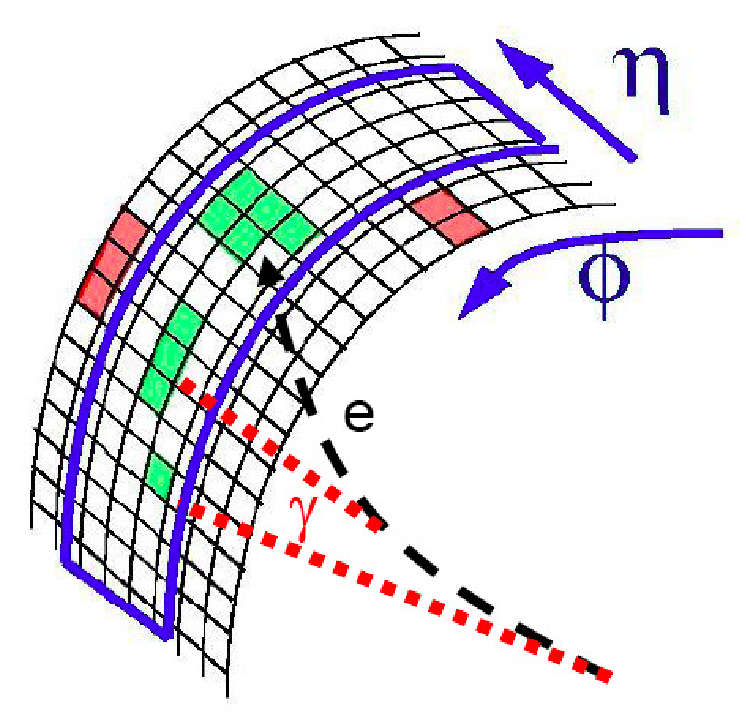
\includegraphics[width=0.3\textwidth]{figures/cms/sc.png}
        \caption{The combination of multiple ECAL crystals into a single supercluster, intended to capture energy depositions from bremsstrahlung photons.
                  Reprinted from Reference~\cite{cmsecalrev}.}
        \label{fig:cms:sc}
    \end{center}
\end{figure}

\subsubsection{Hadronic calorimeter}

\subsubsection{Muon chambers}

\subsubsection{Online trigger system}

\section{Particle reconstruction and identification}

\subsubsection{Particle flow algorithm}

Because of the excellent angular granularity of the CMS detector and the momentum resolution of the tracker, a particle flow~\cite{cmspf} algorithm is used to correlate information from all detector subsystems to build a global description of each event.
Particle flow (PF) algorithms date back to ALEPH~\needcite, and are in contrast to detector-specific physics object-based algorithms used at other experiments (e.g. References~\needcite).

The key feature of the PF algorithm is to ``link'' multiple detector signals together into a single PF candidate.
This linkage combines inner tracks, ECAL clusters, HCAL clusters, and muon tracks based on their proximity in the $(\eta,\phi)$ plane.
Inner track helices are extended into the calorimeters, searching for clusters compatible with the trajectory.
Similarly, clusters from the ECAL, the ECAL preshower, and the HCAL can be linked without a track present. 


\subsubsection{Muons}


\subsubsection{Electrons and photons}

Both electrons and photons are seeded using ECAL SCs, with electrons also being associated with an isolated track.
Due to the significant material budget of the silicon tracker, electrons will lose a significant amount of energy through bremsstrahlung.
Although this energy is partially recovered through the supercluster algorithm, the standard Kalman filter tracking fit does not properly account for the non-Gaussian hit uncertainties induced by bremsstrahlung.
Therefore, a modified algorithm based on a Gaussian Sum Filter (GSF)~\cite{cmstracker,gsf} is used to fit the track.
Hits in the pixel and strip endcap layers consistent with the ECAL SC are used to seed the GSF fit.
GSF differs from a Kalman filter by modeling the uncertainties as a Gaussian mixture model instead of a single Gaussian.
The primary backgrounds for electron identification are (1) the overlap of a charged hadron with a neutral hadron or photon and (2) a photon which converts into a $e^-/e^+$ pair in the tracker.
Table~\ref{tab:cms:el} lists the observables used to reject these backgrounds; two cut-based IDs are defined.
The ``loose'' ID selects electrons with $\sim90\%$ signal efficiency and $\sim0.5\%$ background acceptance (strongly dependent on the electron phase space); it is used to \emph{veto} electrons. 
The ``tight'' ID selects electrons with $\sim70\%$ signal efficiency and $\sim0.1\%$ background acceptance; it is used to \emph{select} electron-pure samples. 

\begin{table}
	\begin{center}
		\caption{Observables used in identifying electrons and rejecting hadron and photon backgrounds}
		\label{tab:cms:el}
		\begin{tabular}{c|p{0.65\textwidth}}
			Observable & Notes \\ 
			\hline
			\hline
			\pt & Backgrounds grow at low \pt~and brem.~photons can make low-\pt~tracking difficult. \\ \hline
			$\sigma_{i\eta i\eta}$  & Energy-weighted width of cell $\eta$ in SC. Small for electrons. \\ \hline
			$|\Delta\eta(\mathrm{track,SC})|$  & $\Delta\eta$ between SC seed crystal and GSF track at PV. Small for electrons.  \\ \hline
			$|\Delta\phi(\mathrm{track,SC})|$  & $\Delta\phi$, as above.\\ \hline
			$E_\mathrm{H}/E_\mathrm{EM}$  & Ratio of HCAL and ECAL energies. Large for hadrons. \\ \hline
			PF isolation & Sum of energies of other PF candiates near electron. Large for particles in jets. \\ \hline
			$|\nicefrac{1}{E}-\nicefrac{1}{p}|$ & Checks if ECAL and tracker agree ($m_e\sim0$) \\ \hline
			$N_\mathrm{hit}^\mathrm{miss}$ & Conversions or bad tracks will have multiple missing hits in the inner tracker.\\ \hline
			Conversion veto & Check for a pair of tracks originating at a displaced vertex.\\ 
		\end{tabular}
	\end{center}
\end{table}

Photons are defined as ECAL SCs without matched tracks. 
Table~\ref{tab:cms:pho} describes the selection variables used to define the loose veto ID ($\epsilon_\mathrm{sig}\approx90\%$, $\epsilon_\mathrm{bkg}\approx17\%$) and the tight selection ID ($\epsilon_\mathrm{sig}\approx82\%$, $\epsilon_\mathrm{bkg}\approx12\%$).
The direction and energy of a photon are defined by the ECAL SC position and energy, respectively.

\begin{table}
	\begin{center}
		\caption{Observables used in identifying photons and rejecting hadron backgrounds}
		\label{tab:cms:pho}
		\begin{tabular}{c|p{0.65\textwidth}}
			Observable & Notes \\ 
			\hline
			\hline
			\pt & Backgrounds grow at low \pt. \\ \hline
			$\eta$ & EB resolution is better than EE; less hadron background. \\ \hline
			$\sigma_{i\eta i\eta}$  & Defined in Table~\ref{tab:cms:el}. \\ \hline
			$E_\mathrm{H}/E_\mathrm{EM}$  & Defined in Table~\ref{tab:cms:el}. \\ \hline
			PF isolations & Defined in Table~\ref{tab:cms:el}. For photons, separate isolation criteria are placed on each PF type (photon, charged hadron, neutral hadron). \\ 
		\end{tabular}
	\end{center}
\end{table}

To calibrate ECAL SCs, we define the $R_9 = E_{3\times3}/E_\mathrm{SC}$. 
$E_{3\times3}$ is the sum of the energies of the crystals in a $3\times3$ square centered on the most energetic crystal in the SC. 
Much like $\sigma_{i\eta i\eta}$, it is sensitive to the width of the shower shape.
A regression to correct the energy scale~\cite{cmsecalreco} is trained as a function of SC energy, $\eta$, $R_9$, and the width of the SC in $\phi$.
To account for differences between data and simulation in the performance of the electron and photon IDs, corrections (known as scale factors) are derived:
\begin{equation}
	\SF = \frac{\epsilon_\mathrm{Data}}{\epsilon_\mathrm{MC}}
\end{equation}
While $\epsilon_\mathrm{MC}$ can be computed directly from MC truth information, $\epsilon_\mathrm{Data}$ must be computed from $Z\rightarrow ee$ events, using one electron as a reference tag, and the other to probe the efficiency of the ID being tested.
In the case of the photon ID, the electron SC is used as a proxy for the photon.

\subsubsection{Jets}
\label{sec:cms:jets}

\subsubsection{Hadronic taus}

\subsubsection{Missing momentum}
\label{sec:cms:met}


\section{Simulation of collisions}

\subsection{Physics simulation}

\subsection{Detector simulation}
